% CVPR 2027 submission — GenAU.
% Ported from the ICLR 2027 version (this same directory, before the rename) and,
% for the two-column scaffolding, from the WACV 2027 version in ../GenAU.
% See PORTING_NOTES.md.
%
% Build: pdflatex main -> bibtex main -> pdflatex main -> pdflatex main -> pdflatex main
% (the third pass after bibtex is needed for the pagebackref lists to settle)
%
% TEMPLATE: cvpr.sty is the official CVPR 2027 author kit file (tag CVPR2027-v1,
% github.com/cvpr-org/author-kit, released 2026-10-28). The 2027 review format no
% longer prints a paper ID, so \paperID is not defined.
\documentclass[10pt,twocolumn,letterpaper]{article}

%%%%%%%%% PAPER TYPE  - PLEASE UPDATE FOR FINAL VERSION
\usepackage[review]{cvpr}      % To produce the REVIEW version
% \usepackage{cvpr}              % To produce the CAMERA-READY version
% \usepackage[pagenumbers]{cvpr} % To force page numbers, e.g. for an arXiv version

% Import additional packages in the preamble file, before hyperref
%
% CVPR preamble.
%
% cvpr.sty already provides: times, xspace, xcolor[dvipsnames], graphicx,
% amsmath, amssymb, booktabs, natbib[numbers,sort&compress], silence, etoolbox,
% caption, subcaption, url and enumitem -- and it loads cleveref itself via
% \AtEndPreamble (i.e. strictly after hyperref), so none of those may be loaded
% here. (This is the same package set wacv.sty supplied; the ICLR port had to
% declare them all by hand because iclr2027_conference.sty supplied only
% fancyhdr + natbib.)
%
% Disable PDF object-stream compression: the large architecture figure this
% was added for (the former imgs/GenAU_Arch_final.pdf) otherwise overflowed pdfTeX's
% object-stream buffer ("TeX capacity exceeded [PDF object stream buffer]").
\ifdefined\pdfobjcompresslevel \pdfobjcompresslevel=0 \fi

% --- required by this paper and NOT provided by cvpr.sty ---
\usepackage{multirow}   % \multirow in the result/ablation tables
\usepackage{colortbl}   % \rowcolor{gray!20} (the "table" feature of xcolor)
\usepackage{tikz}       % motivation radar chart (Fig. 1)
\usepackage{microtype}  % char protrusion + font expansion: tighter lines, fewer runts

% --- compact (but standard) float spacing to help fit the page limit ---
\setlength{\textfloatsep}{10pt plus 2pt minus 2pt}      % top/bottom single-col floats
\setlength{\intextsep}{10pt plus 2pt minus 2pt}         % [h] floats
\setlength{\dbltextfloatsep}{12pt plus 2pt minus 2pt}   % full-width figure*/table*

% --- inline annotations
\newcommand{\red}[1]{{\color{red}#1}}
\newcommand{\todo}[1]{{\color{red}#1}}
\newcommand{\TODO}[1]{\textbf{\color{red}[TODO: #1]}}
% --- disable by uncommenting
% \renewcommand{\TODO}[1]{}
% \renewcommand{\todo}[1]{#1}


% hyperref with pagebackref eases the reviewers' job. cvpr.sty loads cleveref
% itself (\AtEndPreamble, i.e. strictly after hyperref), so do NOT load it here.
\definecolor{cvprblue}{rgb}{0.21,0.49,0.74}
\usepackage[pagebackref,breaklinks,colorlinks,allcolors=cvprblue]{hyperref}

\def\confName{CVPR}
\def\confYear{2027}

%%%%%%%%% TITLE - PLEASE UPDATE
% "Language-Grounded" = localization read out from tokens generated within the textual response
% (defined in sec/1_intro.tex), NOT that linguistic semantics drive localization -- the
% learned-query control does not support that stronger reading (Appendix, app:anchors).
\title{GenAU: Language-Grounded Industrial Anomaly Understanding with One Vision-Language Model}

%%%%%%%%% AUTHORS - PLEASE UPDATE
% CVPR review submissions are double-blind. With \usepackage[review]{cvpr} the
% style prints "Anonymous CVPR submission" instead of this
% block, so it only matters for the camera-ready.
\author{First Author\\
Institution1\\
Institution1 address\\
{\tt\small firstauthor@i1.org}
% For a paper whose authors are all at the same institution,
% omit the following lines up until the closing ``}''.
% Additional authors and addresses can be added with ``\and'',
% just like the second author.
% To save space, use either the email address or home page, not both
\and
Second Author\\
Institution2\\
First line of institution2 address\\
{\tt\small secondauthor@i2.org}
}

\begin{document}
\maketitlesupplementary
% Supplementary floats use an "A" prefix (Table A1, Figure A1) so they are never
% confused with the main paper's tables and figures. References to the main paper
% are written as plain text ("Table 1 of the main paper"), not \ref.
\renewcommand{\thetable}{A\arabic{table}}
\renewcommand{\thefigure}{A\arabic{figure}}
\appendix

\section{Datasets}
\label{app:datasets}
Due to space limitations in the main manuscript, we provide here a detailed description of the industrial anomaly detection datasets used in our experiments: MVTec-AD~\cite{Bergmann_2019_CVPR}, VisA~\cite{VisA}, MPDD~\cite{mpdd}, and Real-IAD~\cite{wang2024realiadrealworldmultiviewdataset}. \Cref{tab:dataset_summary} summarizes, for each split we use, the number of objects, normal and anomalous images, and defect classes.
MVTec-AD includes common industrial items such as bottles, cables, zippers, and hazelnuts. VisA contains a mixture of everyday products such as chewing gum and macaroni, as well as more complex components like printed circuit boards. MPDD focuses primarily on industrial parts, including metal brackets, tubes, and machined components. Real-IAD contains a broad range of real-world consumer and industrial items such as audio jacks, switches, bottle caps, and plastic toys. MVTec-AD is the training source; VisA, MPDD, and Real-IAD are the evaluation targets for binary detection and segmentation, and VisA and MPDD also for defect-type recognition, using the per-object taxonomy of Sec.~\ref{app:taxonomy}.

For defect reasoning we use VisA-D\&R~\cite{xu2025towards}, which pairs $1{,}000$ anomalous VisA images with multi-turn questions and reference answers. The first question of each conversation asks for a description of the anomaly (low-level perception), and the following questions ask about its significance, likely cause, and prevention (complex reasoning).

% Overview of Datasets
\begin{table}[t]
\centering
\footnotesize
\setlength{\tabcolsep}{4pt}
\caption[Overview of the datasets.]{Overview of the datasets. Image counts refer to the splits we use: the MVTec-AD test split for training, and the test splits of VisA, MPDD, and Real-IAD (single view) for evaluation. \emph{Classes} counts the distinct defect labels of the taxonomy in Sec.~\ref{app:taxonomy}, excluding the \emph{combined} class; Real-IAD keeps its native labels.}
\label{tab:dataset_summary}
\begin{tabular}{@{}llrrrr@{}}
\toprule
\textbf{Dataset} & \textbf{Role} & \textbf{Objects} & \textbf{Normal} & \textbf{Anomalous} & \textbf{Classes} \\
\midrule
MVTec-AD  & source & 15 & 467      & 1{,}258 & 20 \\
VisA      & target & 12 & 962      & 1{,}200 & 18 \\
MPDD      & target & 6  & 176      & 282     & 6  \\
Real-IAD  & target & 30 & 10{,}387 & 9{,}415 & 8  \\
\bottomrule
\end{tabular}
\end{table}

\section{Implementation Details}
\label{app:impl}
We build GenAU on the LLaVA-OneVision family~\cite{li2025llavaonevision}, which couples a Qwen2 language backbone with a SigLIP-so400m-patch14-384 vision encoder, and report the 0.5B and 7B scales. High-resolution inputs use the AnyRes scheme (\texttt{anyres\_max\_9}) with an image grid of up to $6\times6$ tiles of $384$ pixels, in addition to a global low-resolution view. For the segmentation readout we take patch features from four vision-encoder stages (layers $6$, $12$, $18$, and the final layer) and equip each stage with its own linear projection into the decoder hidden space.

\paragraph{Trainable parameters.}
The vision encoder is frozen; the cross-modal projector is trained with a learning rate of $10^{-4}$. The LLM is adapted with rank-stabilized LoRA (rank $r=16$, $\alpha=32$, dropout $0$). The token-embedding table and language-modeling head are fully fine-tuned to integrate the two added segmentation tokens \texttt{[SEG\_normal]} and \texttt{[SEG\_defect]}, and the four segmentation projectors together with the decoder layer-norms are trainable.

\paragraph{Optimization.}
Training runs for a single epoch with an effective batch size of $32$ (per-device batch $1$, gradient accumulation $4$, across $8$ GPUs with DeepSpeed ZeRO-3), a learning rate of $10^{-4}$ with cosine decay, a warmup ratio of $0.03$, and no weight decay. The segmentation objective sums, over the four stages, a focal term on the upsampled logits, a Tversky term ($\alpha=0.3$, $\beta=0.7$) on the defect channel that up-weights false negatives, and a Dice term on the complementary normal channel; the text and segmentation losses are weighted equally ($\lambda_{\mathrm{seg}}=1$).

\paragraph{High-resolution readout and image-level fusion.}
At inference the high-resolution and global-view anomaly maps are fused per stage as $\mathbf{A}=(1-\omega)\,\mathbf{A}^{\mathrm{g}}+\omega\,\mathbf{A}^{\mathrm{hi}}$ with $\omega=0.25$ and a similarity temperature of $20$. The image-level score fuses the spatial maximum of $\mathbf{A}$ with the decoder's normal/defect log-odds, averaged over eight phrasings of the yes/no question (generic templates that name only the object category and carry no defect information: ``Is the \{obj\} intact, or are there any anomalies?'', ``Is there anything unusual about the \{obj\} in the image?'', ``Can you identify any defects on the \{obj\}?'', ``Does the \{obj\} shown in the image have any defect?'', ``Is there any anomaly on the \{obj\}?'', ``Inspect the \{obj\}: are there any anomalies present?'', ``Are there any visible anomalies on the \{obj\}?'', and ``Do you see any surface defects on the \{obj\}?''; the image prefix is encoded once and its cache reused for each phrasing). The two are each $z$-score standardized with statistics estimated once on the MVTec-AD source images and averaged with equal weights; the standardization is frozen and shared across target datasets, so no target-domain labels are used. If a generated answer omits the two segmentation tokens, they are appended to it and their hidden states are read with one additional forward pass, so every test image receives a defect map.

\section{Training Data Construction}
\label{app:data}
The segmentation instruction data for the reported cross-dataset experiments use MVTec-AD~\cite{Bergmann_2019_CVPR} as the source benchmark. We retain its images and masks and add instruction--response pairs. Each sample consists of an image, mask, instruction, and response; the instruction, phrased in several ways, asks whether the named object contains an anomaly and requests localization, e.g.\ \texttt{``Is there any anomaly on the \{object\}? If yes, segment it.''}

The response describes the anomaly in natural language and terminates with the two segmentation tokens \texttt{[SEG\_defect]} and \texttt{[SEG\_normal]}, from which the localization read-out is taken. For a normal image, the response states that no anomaly is present and likewise ends with the two tokens, so that its all-zero mask provides negative supervision. An example response is:

\textit{``Yes, there is an anomaly on the capsule. Specifically, there is a dent on the orange side, affecting the clarity and smoothness of the numeral `0' in the printed number `500.' [SEG\_defect] [SEG\_normal]''}

\paragraph{Reasoning conversations.} For $863$ of the $1{,}725$ training images (drawn at random), the single exchange is replaced by a multi-turn conversation about the same image from the instruction data of Anomaly-OV~\cite{xu2025towards}: an image description, the segmentation request above (answered with the two segmentation tokens), and three to nine follow-up questions, which for anomalous images cover the defect's appearance, significance, likely cause, and prevention. The remaining $862$ images keep the single segmentation exchange. Every image appears exactly once, so the number of samples and optimization steps ($53$ at batch size $32$) matches segmentation-only training. Adding the conversations as extra samples instead (the full reasoning mix of Table~2 of the main paper) doubles the number of steps and lowers detection and localization.

\section{Defect Taxonomy}
\label{app:taxonomy}
Industrial AD datasets often define highly specific defect categories, which can lead to overfitting and inconsistent label usage~\cite{mokhtar2025detectclassifyactcategorizing}. For conditional defect-type recognition we therefore adopt the per-object taxonomy of MultiADS~\cite{sadikaj2025multiadsdefectawaresupervisionmultitype}, which maps product-specific labels to coarser classes: e.g., \textit{broken large} and \textit{broken small} are unified as \textit{broken}, and \textit{different colour spot} and \textit{similar colour spot} as \textit{spot}. The taxonomy is defined per object, so the candidate defect set differs across product categories; each VisA object additionally has a \emph{combined} class for compound defects. The taxonomy defines the candidate labels and the ground truth of the type-recognition evaluation (Sec.~\ref{app:eval}). GenAU is not trained to output taxonomy labels: its training responses name and describe defects in natural language (Sec.~\ref{app:data}). Binary detection and segmentation are independent of class granularity, so comparisons with prior binary methods are unaffected. \Crefrange{tab:mvtec-mapping1}{tab:mpdd-mapping} give the complete per-object mapping for the source dataset MVTec-AD, which shows which target classes also occur among the source defects, and for the two type-recognition targets, VisA and MPDD.

\begin{table}
\centering
\footnotesize
\caption{Defect taxonomy for MVTec-AD (Part I).}
\label{tab:mvtec-mapping1}
\begin{tabular}{@{}ccc@{}}
\toprule
\textbf{Product} & \textbf{Original Defect Type} & \textbf{Mapped Label} \\
\midrule
\multirow{3}{*}{Bottle} & Broken Large & Broken \\
 & Broken Small & Broken \\
 & Contamination & Contamination \\
\midrule
\multirow{8}{*}{Cable} & Bent Wire & Bent \\
 & Cable Swap & Misplaced \\
 & Cut Inner Insulation & Cut \\
 & Cut Outer Insulation & Cut \\
 & Missing Cable & Missing \\
 & Missing Wire & Missing \\
 & Poke Insulation & Poke \\
 & Combined & Combined \\
\midrule
\multirow{5}{*}{Capsule} & Crack & Crack \\
 & Faulty Imprint & Faulty Imprint \\
 & Poke & Poke \\
 & Scratch & Scratch \\
 & Squeeze & Squeeze \\
\midrule
\multirow{5}{*}{Carpet} & Color & Color \\
 & Cut & Cut \\
 & Hole & Hole \\
 & Metal Contamination & Contamination \\
 & Thread & Thread \\
\midrule
\multirow{5}{*}{Grid} & Bent & Bent \\
 & Broken & Broken \\
 & Glue & Glue \\
 & Metal Contamination & Contamination \\
 & Thread & Thread \\
\midrule
\multirow{4}{*}{Hazelnut} & Crack & Crack \\
 & Cut & Cut \\
 & Hole & Hole \\
 & Print & Faulty Imprint \\
\midrule
\multirow{5}{*}{Leather} & Color & Color \\
 & Cut & Cut \\
 & Fold & Misplaced \\
 & Glue & Glue \\
 & Poke & Poke \\
\midrule
\multirow{4}{*}{Metal Nut} & Bent & Bent \\
 & Color & Color \\
 & Flip & Misplaced \\
 & Scratch & Scratch \\
\midrule
\multirow{7}{*}{Pill} & Color & Color \\
 & Contamination & Contamination \\
 & Crack & Crack \\
 & Faulty Imprint & Faulty Imprint \\
 & Pill Type & Damaged \\
 & Scratch & Scratch \\
 & Combined & Combined \\
\midrule
\multirow{5}{*}{Screw} & Manipulated Front & Bent \\
 & Scratch Head & Scratch \\
 & Scratch Neck & Scratch \\
 & Thread Side & Thread \\
 & Thread Top & Thread \\
\bottomrule
\end{tabular}
\end{table}

\begin{table}
\centering
\footnotesize
\caption{Defect taxonomy for MVTec-AD (Part II).}
\label{tab:mvtec-mapping2}
\begin{tabular}{@{}ccc@{}}
\toprule
\textbf{Product} & \textbf{Original Defect Type} & \textbf{Mapped Label} \\
\midrule
\multirow{5}{*}{Tile} & Crack & Crack \\
 & Glue Strip & Glue \\
 & Gray Stroke & Damaged \\
 & Oil & Liquid \\
 & Rough & Rough \\
\midrule
\multirow{1}{*}{Toothbrush} & Defective & Damaged \\
\midrule
\multirow{4}{*}{Transistor} & Bent Lead & Bent \\
 & Cut Lead & Cut \\
 & Damaged Case & Damaged \\
 & Misplaced & Misplaced \\
\midrule
\multirow{5}{*}{Wood} & Color & Color \\
 & Hole & Hole \\
 & Liquid & Liquid \\
 & Scratch & Scratch \\
 & Combined & Combined \\
\midrule
\multirow{7}{*}{Zipper} & Broken Teeth & Broken \\
 & Fabric Border & Fabric \\
 & Fabric Interior & Fabric \\
 & Split Teeth & Misplaced \\
 & Squeezed Teeth & Squeezed \\
 & Rough & Rough \\
 & Combined & Combined \\
\bottomrule
\end{tabular}
\end{table}

\begin{table}
\centering
\footnotesize
\caption{Defect taxonomy for VisA (Part I).}
\label{tab:visa-mapping1}
\begin{tabular}{@{}ccc@{}}
\toprule
\textbf{Product} & \textbf{Original Defect Type} & \textbf{Mapped Label} \\
\midrule
\multirow{8}{*}{Candle} & Chunk of Wax Missing & Missing \\
 & Damaged Corner of Packaging & Damaged \\
 & Different Colour Spot & Spot \\
 & Extra Wax in Candle & Extra \\
 & Foreign Particles on Candle & Particles \\
 & Wax Melded out of the Candle & Melted \\
 & Weird Candle Wick & Weird Wick \\
 & Combined & Combined \\
\midrule
\multirow{2}{*}{Capsules} & Bubble & Bubble \\
 & Combined & Combined \\
\midrule
\multirow{9}{*}{Cashew} & Burnt & Burnt \\
 & Corner or Edge Breakage & Broken \\
 & Middle Breakage & Broken \\
 & Different Colour Spot & Spot \\
 & Same Colour Spot & Spot \\
 & Small Holes & Hole \\
 & Small Scratches & Scratch \\
 & Stuck Together & Stuck \\
 & Combined & Combined \\
\midrule
\multirow{5}{*}{Chewing Gum} & Chunk of Gum Missing & Missing \\
 & Corner Missing & Missing \\
 & Scratches & Scratch \\
 & Similar Colour Spot & Spot \\
 & Combined & Combined \\
\midrule
\multirow{8}{*}{Fryum} & Burnt & Burnt \\
 & Middle Breakage & Broken \\
 & Corner or Edge Breakage & Broken \\
 & Different Colour Spot & Spot \\
 & Similar Colour Spot & Spot \\
 & Fryum Stuck Together & Stuck \\
 & Small Scratches & Scratch \\
 & Combined & Combined \\
\bottomrule
\end{tabular}
\end{table}

\begin{table}
\centering
\footnotesize
\caption{Defect taxonomy for VisA (Part II).}
\label{tab:visa-mapping2}
\begin{tabular}{@{}ccc@{}}
\toprule
\textbf{Product} & \textbf{Original Defect Type} & \textbf{Mapped Label} \\
\midrule
\multirow{6}{*}{Macaroni1} & Chip Around Edge and Corner & Chip \\
 & Different Colour Spot & Spot \\
 & Similar Colour Spot & Spot \\
 & Small Cracks & Crack \\
 & Small Scratches & Scratch \\
 & Combined & Combined \\
\midrule
\multirow{7}{*}{Macaroni2} & Breakage down the Middle & Broken \\
 & Different Color Spot & Spot \\
 & Color Spot Similar to the Object & Spot \\
 & Small Chip Around Edge & Chip \\
 & Small Cracks & Crack \\
 & Small Scratches & Scratch \\
 & Combined & Combined \\
\midrule
\multirow{5}{*}{PCB1} & Bent & Bent \\
 & Melt & Melt \\
 & Missing & Missing \\
 & Scratch & Scratch \\
 & Combined & Combined \\
\midrule
\multirow{5}{*}{PCB2} & Bent & Bent \\
 & Melt & Melt \\
 & Missing & Missing \\
 & Scratch & Scratch \\
 & Combined & Combined \\
\midrule
\multirow{5}{*}{PCB3} & Bent & Bent \\
 & Melt & Melt \\
 & Missing & Missing \\
 & Scratch & Scratch \\
 & Combined & Combined \\
\midrule
\multirow{7}{*}{PCB4} & Burnt & Burnt \\
 & Scratch & Scratch \\
 & Damage & Damaged \\
 & Extra & Extra \\
 & Missing & Missing \\
 & Wrong Place & Wrong Place \\
 & Combined & Combined \\
\midrule
\multirow{7}{*}{Pipe Fryum} & Burnt & Burnt \\
 & Corner and Edge Breakage & Broken \\
 & Different Colour Spot & Spot \\
 & Similar Colour Spot & Spot \\
 & Stuck Together & Stuck \\
 & Small Scratches & Scratch \\
 & Combined & Combined \\
\bottomrule
\end{tabular}
\end{table}

\begin{table}
\centering
\footnotesize
\caption{Defect taxonomy for MPDD.}
\label{tab:mpdd-mapping}
\begin{tabular}{@{}ccc@{}}
\toprule
\textbf{Product} & \textbf{Original Defect Type} & \textbf{Mapped Label} \\
\midrule
\multirow{2}{*}{Bracket Black} & Hole & Hole \\
 & Scratches & Scratch \\
\midrule
\multirow{2}{*}{Bracket Brown} & Parts Mismatch & Mismatch \\
 & Bend and Parts Mismatch & Mismatch \\
\midrule
\multirow{2}{*}{Bracket White} & Defective Painting & Defective Painting \\
 & Scratches & Scratch \\
\midrule
\multirow{1}{*}{Connector} & Parts Mismatch & Mismatch \\
\midrule
\multirow{3}{*}{Metal Plate} & Major Rust & Rust \\
 & Total Rust & Rust \\
 & Scratches & Scratch \\
\midrule
\multirow{1}{*}{Tubes} & Anomalous & Flattening \\
\bottomrule
\end{tabular}
\end{table}

\section{Evaluation Protocol}
\label{app:eval}
All models are evaluated under single-image inference: only the query image is available at test time, with no reference, support, or exemplar images. GenAU is fine-tuned on the MVTec-AD test split (the only MVTec split carrying anomaly masks and defect-type labels, as the train split contains normal images only) and evaluated, without retraining, on the test splits of VisA, MPDD, and Real-IAD; MVTec thus serves purely as the source domain: its images are disjoint from all evaluation targets and no target labels enter training or calibration, although three Real-IAD categories (toothbrush, zipper, transistor) share names with MVTec-AD categories. Design choices were compared on VisA (Table~2 of the main paper and Table~\ref{tab:ablations}), which thus also served as the development target. For Real-IAD we use the single-view setting.

\paragraph{Unified inspection prompt.}
For binary detection and segmentation, the instruction names the object category and asks for an anomaly decision and its localization: \texttt{``Is there any anomaly on the \{object\}? If yes, segment it.''} The model is trained to follow its answer with both segmentation tokens; tokens that generation omits are appended before readout (Sec.~\ref{app:impl}), so every evaluated image receives an anomaly map.

\paragraph{Product-conditioned multi-type detection.}
The reported multi-type table evaluates forced-choice recognition on known-anomalous images. The prompt states that the image contains a defect and lists the object's candidate labels from the taxonomy of Sec.~\ref{app:taxonomy} in alphabetical order: \texttt{``This is an image of a \{object\} that contains a defect. Identify the defect type. Choose exactly one option from this list and answer with only that option, nothing else: \{defect list\}.''} Normal is excluded from both the options and scoring. Images whose original label has no entry in the taxonomy are excluded before evaluation, leaving $916$ VisA images and all $282$ MPDD anomalous images. The \emph{combined} class represents a compound defect as one class; the task does not require recovering multiple independent labels. The supplied object vocabulary is target-domain metadata, not a prediction of the valid vocabulary.

The parser lowercases the response, replaces underscores with spaces, and searches for candidate labels and their mapped fine-label synonyms. The earliest matching substring wins; no match returns \texttt{none}, counted as an incorrect prediction. Weighted precision, recall, and F1 are computed over the pooled images with class-support weights and zero scores for undefined divisions, rather than averaging per-object F1. Every image in each mapped subset has an answer in the reported runs. Normal images are evaluated by the binary detection task.

\paragraph{Single-checkpoint evaluation.}
Every task uses the checkpoint of Table~1 of the main paper, without weight changes. Detection and segmentation use the inspection prompt, type recognition uses the forced-choice prompt, and VisA-D\&R uses its conversational questions.

\paragraph{Reasoning conversations in training.}
Training with reasoning conversations preserves the ability to answer causal questions that segmentation-only training loses. On the complex VisA-D\&R questions, GenAU-7B reaches an SBERT similarity to the reference answers of $0.664$, against $0.576$ for the segmentation-only checkpoint with a frozen projector ($0.635$ versus $0.560$ at 0.5B), whereas on the low-level questions, which ask for a description of the anomaly, the two are comparable ($0.579$ versus $0.590$). Giving every training image a conversation (the full reasoning mix of Table~2 of the main paper) brings no further gain at 7B ($0.571$ low-level, $0.666$ complex) but lowers VisA image-AUROC to $87.0\%$, pixel-AUPRO to $85.8\%$, and type-recognition F1 to $29.0\%$ on VisA and $69.8\%$ on MPDD; our default therefore embeds conversations in half of the training samples. These comparisons use the plain VisA-D\&R questions. Table~4 of the main paper appends GenAU's segmentation request ``If yes, segment it.'' to the first question, so that the same conversation also yields the anomaly map, giving $0.596$/$0.648$ (7B) and $0.562$/$0.634$ (0.5B); with the plain questions, GenAU-7B's similarities ($0.579$/$0.664$) likewise exceed those of Anomaly-OV-7B in that table ($0.565$/$0.629$).

\section{Additional Ablations}
\label{app:ablation}
Table~\ref{tab:ablations} ablates, on MVTec-AD$\rightarrow$VisA, four training choices: the weight of the text loss, the number $m$ of vision-encoder stages supplying the segmentation readout, whether the cross-modal projector is trainable, and whether the vision encoder itself is unfrozen. The ablations use the segmentation-only recipe with a frozen cross-modal projector, which isolates the segmentation pathway from the reasoning data; each row changes a single factor relative to the shaded reference row.

Weighting the text loss five times higher ($5\,\mathcal{L}_{\mathrm{txt}}+\mathcal{L}_{\mathrm{seg}}$) changes little: pixel-AUROC rises by $0.6$, and pixel-AUPRO and image-AUROC each fall by $0.2$ points, so we keep equal weights ($\lambda_{\mathrm{seg}}=1$). Reading out $m=3$ instead of four stages slightly raises the image-level scores ($+0.2$ AUROC, $+0.4$ AP) but lowers both pixel metrics (AUROC $94.9$ vs.\ $95.1$, AUPRO $88.4$ vs.\ $88.7$); the readout is thus robust to the number of stages, and the four-stage default localizes better. Making the cross-modal projector trainable improves both pixel metrics ($+0.5$ AUROC and AUPRO) at a cost of $0.6$ points in image-AUROC; the default recipe trains it because, with reasoning conversations in the training data, the trainable projector preserved localization in our development runs. Finally, unfreezing the vision encoder is markedly harmful, lowering pixel-AUPRO to $81.8$ and image-AUROC to $75.6$, far below every other configuration, as the encoder over-fits the small source set; keeping it frozen preserves its pretrained visual features.

\begin{table}[h]
\centering
\small
\setlength{\tabcolsep}{3pt}
\caption{Ablation of single training factors on MVTec-AD$\rightarrow$VisA. The shaded row is the segmentation-only GenAU-7B with a frozen projector ($m{=}4$, $\lambda_{\mathrm{seg}}{=}1$, vision encoder frozen); each subsequent row changes one factor. The ``projector trainable'' row is the ``segmentation only'' row of Table~2 of the main paper. Image columns use the fused score of Table~1 of the main paper. All metrics in \%.}
\label{tab:ablations}
\begin{tabular}{@{}l|cc|cc@{}}
\toprule
 & \multicolumn{2}{c|}{\textbf{Pixel}} & \multicolumn{2}{c}{\textbf{Image}} \\
\cmidrule(lr){2-3}\cmidrule(lr){4-5}
 & AUROC & AUPRO & AUROC & AP \\
\midrule
\rowcolor{gray!20}
seg.\ only, frozen projector & 95.1 & 88.7 & 90.5 & 91.9 \\
\midrule
\quad text-loss weight $5$    & 95.7 & 88.5 & 90.3 & 91.9 \\
\quad $m = 3$ stages          & 94.9 & 88.4 & 90.7 & 92.3 \\
\quad projector trainable     & 95.6 & 89.2 & 89.9 & 91.5 \\
\quad vision encoder unfrozen & 94.4 & 81.8 & 75.6 & 79.7 \\
\bottomrule
\end{tabular}
\end{table}

\subsection{Decoder-Conditioned versus Learned-Query Anchors}
\label{app:anchors}
On the segmentation-only recipe with a frozen projector, we replace the two decoder-conditioned anchors with randomly initialized, trainable constant queries, keeping the trainable segmentation projection and matched inference. Both arms receive maps for every image; omitted segmentation tokens in the decoder arm are appended before readout. The queries are learned during training, not fixed random vectors at test time. The control thus compares anchors conditioned on the image, instruction, and response with context-free learned queries.

Table~\ref{tab:anchor_seeds} reports pixel-AUPRO for seeds $42$, $43$, and $44$ on all three targets. On VisA, decoder anchors lead in every seed, by $4.40$ points on average. On MPDD and Real-IAD, the two arms are close on average (differences of $-0.47$ and $-0.68$ points, smaller than the seed standard deviations), so the mean localization benefit is dataset-dependent. Decoder anchors are, however, more stable on all three targets: they show the smaller spread across seeds (standard deviation $0.81$, $1.02$, and $1.27$ versus $6.10$, $1.44$, and $3.94$ points) and the higher worst-seed AUPRO ($87.70$, $87.11$, and $85.38$ versus $77.13$, $86.58$, and $82.80$), whereas learned queries drop by $7$--$11$ points in one seed on VisA and on Real-IAD. The decoder arm also provides the seed variability referred to in Table~1 of the main paper: across the three seeds, the pixel-AUPRO of this segmentation-only recipe varies with a standard deviation of $0.8$--$1.3$ points.

\begin{table}[t]
\centering
\small
\setlength{\tabcolsep}{3pt}
\caption{Matched anchor controls: pixel-AUPRO (\%). Mean rows give mean $\pm$ sample standard deviation across three seeds; $\Delta$ is decoder minus learned-query AUPRO in percentage points.}
\label{tab:anchor_seeds}
\begin{tabular}{@{}llrrr@{}}
\toprule
\textbf{Dataset} & \textbf{Seed} & \textbf{Decoder} & \textbf{Learned} & $\boldsymbol{\Delta}$ \\
\midrule
VisA & 42 & 88.66 & 87.38 & $+1.28$ \\
  & 43 & 87.70 & 77.13 & $+10.57$ \\
  & 44 & 89.32 & 87.99 & $+1.33$ \\
  & Mean & $88.56\pm0.81$ & $84.16\pm6.10$ & $+4.40$ \\
\midrule
MPDD & 42 & 88.91 & 88.73 & $+0.19$ \\
  & 43 & 87.16 & 86.58 & $+0.59$ \\
  & 44 & 87.11 & 89.31 & $-2.19$ \\
  & Mean & $87.73\pm1.02$ & $88.20\pm1.44$ & $-0.47$ \\
\midrule
Real-IAD & 42 & 87.93 & 89.71 & $-1.78$ \\
      & 43 & 86.69 & 82.80 & $+3.89$ \\
      & 44 & 85.38 & 89.53 & $-4.15$ \\
      & Mean & $86.67\pm1.27$ & $87.35\pm3.94$ & $-0.68$ \\
\bottomrule
\end{tabular}
\end{table}

\section{Formal Task Definitions}
\label{app:tasks}
We give the full definitions of the three tasks summarized in Section~3 of the main paper.

\paragraph{Binary anomaly detection under distribution shift.}
Let $\mathcal{D}_{\text{train}}=\{(\boldsymbol{x}_i,y_i)\}_{i=1}^{N_1}$ and $\mathcal{D}_{\text{target}}=\{(\boldsymbol{x}_i,y_i)\}_{i=N_1+1}^{N_1+N_2}$ be two image--label datasets drawn from different input distributions $\mathcal{P}(\mathcal{X}),\mathcal{P}(\mathcal{X}')$: $\forall i\in\{1,\dots,N_1\}$, $\boldsymbol{x}_i\sim\mathcal{P}(\mathcal{X})$, and $\forall i\in\{N_1+1,\dots,N_1+N_2\}$, $\boldsymbol{x}_i\sim\mathcal{P}(\mathcal{X}')$, where $\mathcal{P}(\mathcal{X})\nsim\mathcal{P}(\mathcal{X}')$. Each image $\boldsymbol{x}\in\mathbb{R}^{H\times W\times 3}$ is labeled with $y\in\{0,1\}$, where $y=1$ indicates that it contains at least one anomaly. A binary detector $\hat{f}(\cdot)$ is trained solely on $\mathcal{D}_{\mathrm{train}}$ and applied to $\mathcal{D}_{\mathrm{target}}$ without retraining; at test time it may additionally be conditioned on target-domain metadata such as a product description, but not on target labels. For each $\boldsymbol{x}\in\mathcal{D}_{\mathrm{target}}$, it outputs an anomaly score $s(\boldsymbol{x})\in\mathbb{R}$ and classifies the image as normal or anomalous by thresholding it.

\paragraph{Binary anomaly segmentation under distribution shift.}
With $\mathcal{D}_{\text{train}}$ and $\mathcal{D}_{\text{target}}$ as above and $\mathcal{P}(\mathcal{X})\nsim\mathcal{P}(\mathcal{X}')$, each image $\boldsymbol{x}\in\mathbb{R}^{H\times W\times 3}$ is paired with a binary mask $\boldsymbol{y}\in\{0,1\}^{H\times W}$ indicating the presence of anomalies at each pixel; normal images have an all-zero mask. The segmentation model $\hat{f}(\cdot)$ is trained solely on $\mathcal{D}_{\mathrm{train}}$ and applied without retraining, optionally conditioned on target-domain metadata. For each $\boldsymbol{x}\in\mathcal{D}_{\mathrm{target}}$, it produces an anomaly map $\mathbf{A}\in\mathbb{R}^{H\times W}$ and classifies each pixel as normal or anomalous by thresholding the map.

\paragraph{Conditional defect-type recognition under distribution shift.}
For a known-anomalous target image $\boldsymbol{x}$ of object $o$, the supplied candidate set $C_{\mathrm{target}}(o)$ contains mapped coarse defect labels, including compound classes where defined. The target label is one member $y'\in C_{\mathrm{target}}(o)$, and the model predicts one label through conditional generation and parsing. The target vocabulary mixes labels seen in source training and novel labels; normal images and unmapped defect labels are outside this conditional evaluation. This setting tests cross-dataset type recognition with a supplied vocabulary, not arbitrary multi-label prediction or discovery of the target taxonomy.

\section{Extended Related Work}
\label{app:related}
This expands the related-work overview of the main text.

\paragraph{CLIP-based prompt adaptation for anomaly detection and segmentation.}
Recent advances in industrial anomaly detection/segmentation have largely built upon CLIP due to its strong zero-shot transfer ability, although CLIP was not originally designed for industrial inspection. A major line of work adapts CLIP to industrial AD through normal/abnormal prompts, learnable prompt tokens, or improved visual--text alignment. WinCLIP~\cite{jeong2023winclip} introduces normal and abnormal textual prompts together with window-based feature aggregation for zero-shot anomaly detection. AnomalyCLIP~\cite{zhou2024anomalyclip} learns object-agnostic prompts to capture generic semantics of normality and abnormality, while PromptAD~\cite{Li_2024_WACV} improves state discrimination by adding learnable prefix and suffix tokens. AdaCLIP~\cite{Cao_2024} further combines static and dynamic learnable prompts for adaptive inference across object categories. Beyond prompt learning, CLIP-based methods have been extended to localization and segmentation by improving patch-level alignment or incorporating external modules. APRIL-GAN~\cite{chen2023zero}, AnoCLIP~\cite{deng2024}, SimCLIP~\cite{simclip}, VCP-CLIP~\cite{qu2024vcpclip}, and AA-CLIP~\cite{ma2025aaclip} enhance cross-modal alignment for pixel-level anomaly mapping, while CLIP-SAM~\cite{li2024clipsamclipsamcollaboration} and FiLo~\cite{gu2024filozeroshotanomalydetection} combine CLIP with external segmentation or grounding models, and MultiADS~\cite{sadikaj2025multiadsdefectawaresupervisionmultitype} introduces defect-aware textual supervision for multi-type anomaly detection. Other approaches, such as MuSc~\cite{li2024musczeroshotindustrialanomaly}, MAEDAY~\cite{schwartz2024maeday}, and Aota et al.~\cite{aota2023zero}, rely on patch comparison, feature uniformity, or reconstruction difficulty. Despite their effectiveness, these methods largely depend on CLIP-style embedding comparison, external localization modules, or non-generative anomaly scoring, making them less suited for unified defect reasoning and analysis.

\paragraph{Autoregressive VLMs for anomaly detection and reasoning.}
Autoregressive VLMs provide a different paradigm for anomaly understanding by enabling open-ended visual reasoning and instruction-following interaction. Instead of comparing an image embedding with a fixed set of CLIP prompts, they can generate textual descriptions, answer inspection questions, and reason over defect attributes in natural language. AnomalyGPT~\cite{gu2023anomalygptdetectingindustrialanomalies} is an early effort: it lets users query an instruction-following VLM about industrial anomalies, but its localization map comes from a dedicated image--text matching decoder and is fed to the language model as prompt embeddings, so the VLM reasons over a map it does not itself produce. Myriad~\cite{li2023myriad} likewise injects anomaly maps from vision experts into the model. MMAD~\cite{jiang2025mmad} benchmarks multimodal large language models on industrial inspection questions and finds even strong models well short of industrial requirements, whereas GenAU reads the VLM's yes/no prior out as a calibrated image-level score (Sec.~4.3 of the main paper). More recently, Anomaly-OV~\cite{xu2025towards} specializes multimodal large language models for zero-shot anomaly detection and defect reasoning via Anomaly-Instruct-125k, a large-scale visual instruction-tuning dataset for anomaly-centric understanding; it targets image-level detection and explanation and produces no pixel-level segmentation.

\paragraph{Reasoning segmentation with VLMs.}
LISA~\cite{lai2024lisareasoningsegmentationlarge} introduced reasoning segmentation, in which a VLM emits a segmentation token whose hidden state prompts a mask decoder; GLaMM~\cite{rasheed2024glamm} and PixelLM~\cite{ren2024pixellm} extend this paradigm to grounded conversation and multi-object segmentation. GenAU builds on this paradigm but uses the decoder hidden states of two dedicated tokens, \texttt{[SEG\_normal]} and \texttt{[SEG\_defect]}, as decoder-conditioned anchors that are matched directly against frozen multi-scale visual features, without an external mask decoder, and it unifies image-level anomaly detection, anomaly segmentation, defect-type recognition, and textual defect analysis in one instruction-following model.

\section{Detailed Evaluation Metrics}
\label{app:metrics}
\paragraph{Detection and segmentation.}
For image-level detection we report the area under the receiver operating characteristic curve (AUROC) and the average precision (AP) of the image-level score. For segmentation we report the pixel-level AUROC of the anomaly map and the area under the per-region overlap curve (AUPRO). For a given threshold, the per-region overlap averages, over all annotated defect regions, the fraction of each region covered by the thresholded map; AUPRO integrates it over pixel false-positive rates from $0$ to $0.3$, normalized to that range, so that small and large defects contribute equally.

\paragraph{Defect-type recognition.}
For multi-type detection we use weighted precision, recall, and F1, computed over the pooled images of a dataset: each class's score is weighted by its number of ground-truth images, which accounts for the strong class imbalance across defect categories.

\paragraph{Defect reasoning.}
We follow the VisA-D\&R protocol~\cite{xu2025towards} (Sec.~\ref{app:datasets}), with the first question of each conversation counted as low-level perception and all later questions as complex reasoning. For the GPT-Score, GPT-4o rates each answer against the reference answer on a $1$--$10$ scale, with the same judge prompt for every model. SBERT is the cosine similarity between \texttt{all-MiniLM-L6-v2} sentence embeddings of answer and reference. Both are averaged separately over low-level and complex questions, after removing segmentation tokens from the answers. All models in Table~4 of the main paper, including the baselines, are generated and scored with this same pipeline; published scores are not used.

\section{Qualitative Results}
\label{app:qualitative}
We provide additional anomaly maps of GenAU-7B for five products, each with eight anomalous test images: tubes (\cref{fig:tubes}) from MPDD, capsules (\cref{fig:capsules}) and pipe fryum (\cref{fig:pipe-fryum}) from VisA, and mounts (\cref{fig:mounts}) and rolled strip base (\cref{fig:rolled_strip_base}) from Real-IAD. To avoid best-case selection, the eight images of a product are spread over its defect types and, within each type, over evenly spaced quantiles of the per-image pixel AP (at most one camera view per Real-IAD specimen); each product's maps share one colour scale.

On the tubes, the deformed tube receives the strongest response in most images, while the intact tubes show a weaker, uniform activation. On the capsules, large defects such as leaks and misshapes are localized clearly, but small bubbles and discolorations receive only weak responses, and one map shows a diffuse response over the background. On the pipe fryum, breakage and spots near the edges are localized, while scratches are covered only coarsely and the object surface is moderately activated throughout. On the Real-IAD mounts, missing parts and pits are localized, but a contamination at the inner rim of the hole is missed (first image). On the rolled strip base, the defects are localized, and weaker responses also appear on salient structures such as the screw holes and diagonal ribs, in line with the weak boundary responses noted in Sec.~5.5.1 of the main paper.

\cref{fig:text} shows complete VisA-D\&R conversations, chosen at the class-median GPT-Score rather than as best cases. In the first turn GenAU answers and emits the segmentation tokens; in all three images the strongest response of the resulting map lies on the annotated defect, with weaker responses on the upper lobe of the cashew and on the PCB's LED. The text is less reliable than the maps: GenAU describes the cashew's hole as a dark spot, calls the pipe fryum a pill, and attributes the PCB anomaly to a bent transistor lead, while its own map highlights the excess solder on the potentiometer that the reference names. Once the follow-up question names the defect, the explanations of its significance, causes, and prevention are mostly consistent with the reference, which matches the gap between low-level and complex GPT-Scores in Table~4 of the main paper.

\begin{figure*}
  \centering
  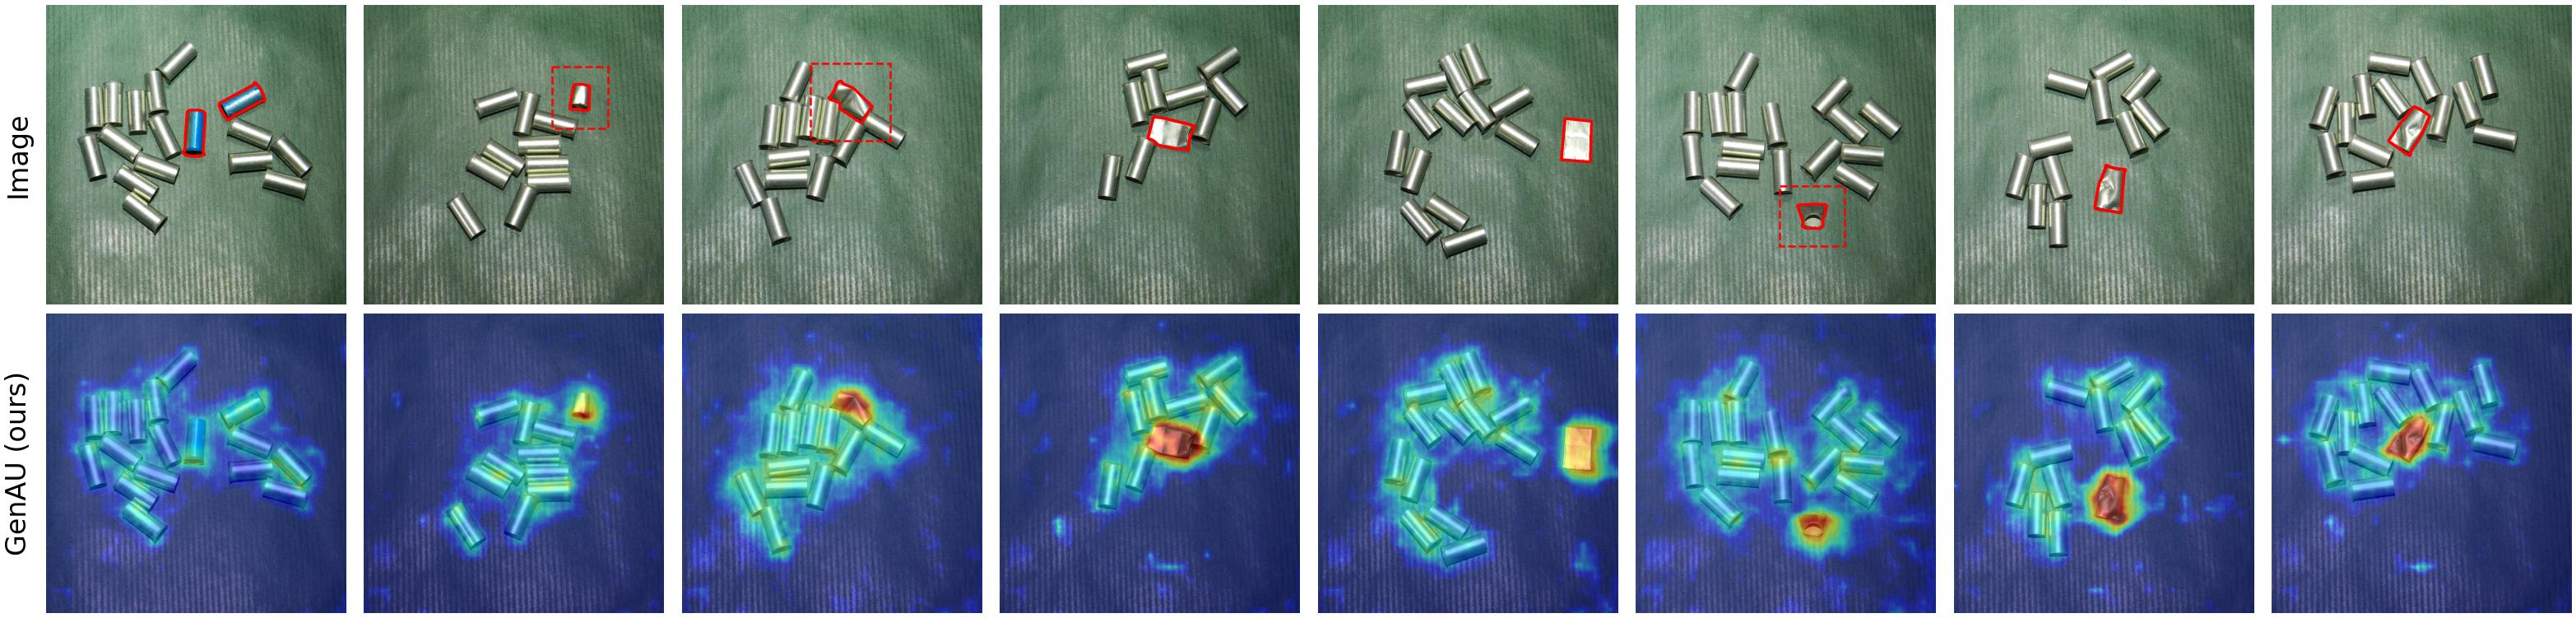
\includegraphics[width=\textwidth]{imgs/tubes.jpg}
  \caption{Tubes (MPDD). Ground truth is outlined in red (small defects are additionally marked with a dashed box); the second row shows the GenAU-7B anomaly maps.}
  \label{fig:tubes}
\end{figure*}

\begin{figure*}
  \centering
  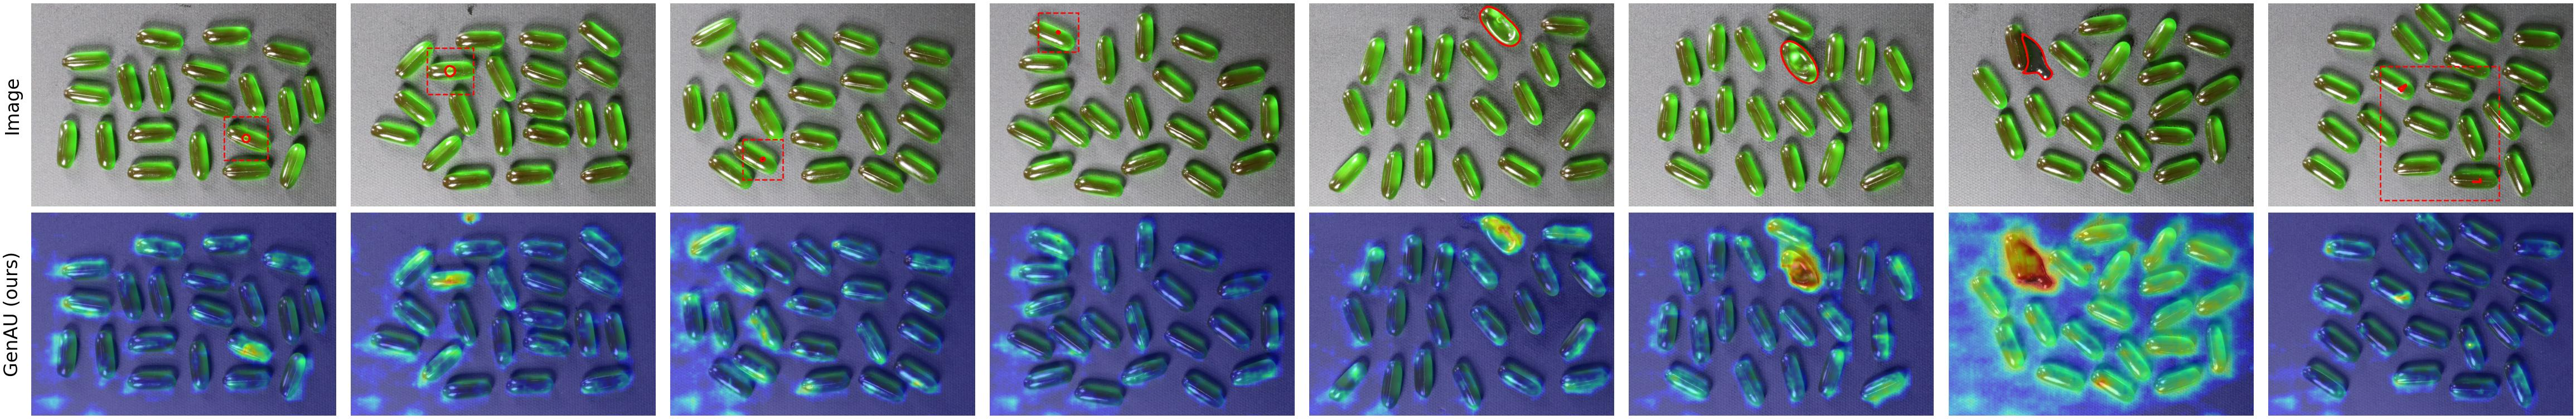
\includegraphics[width=\textwidth]{imgs/capsules.jpg}
  \caption{Capsules (VisA). Ground truth is outlined in red (small defects are additionally marked with a dashed box); the second row shows the GenAU-7B anomaly maps.}
  \label{fig:capsules}
\end{figure*}

\begin{figure*}
  \centering
  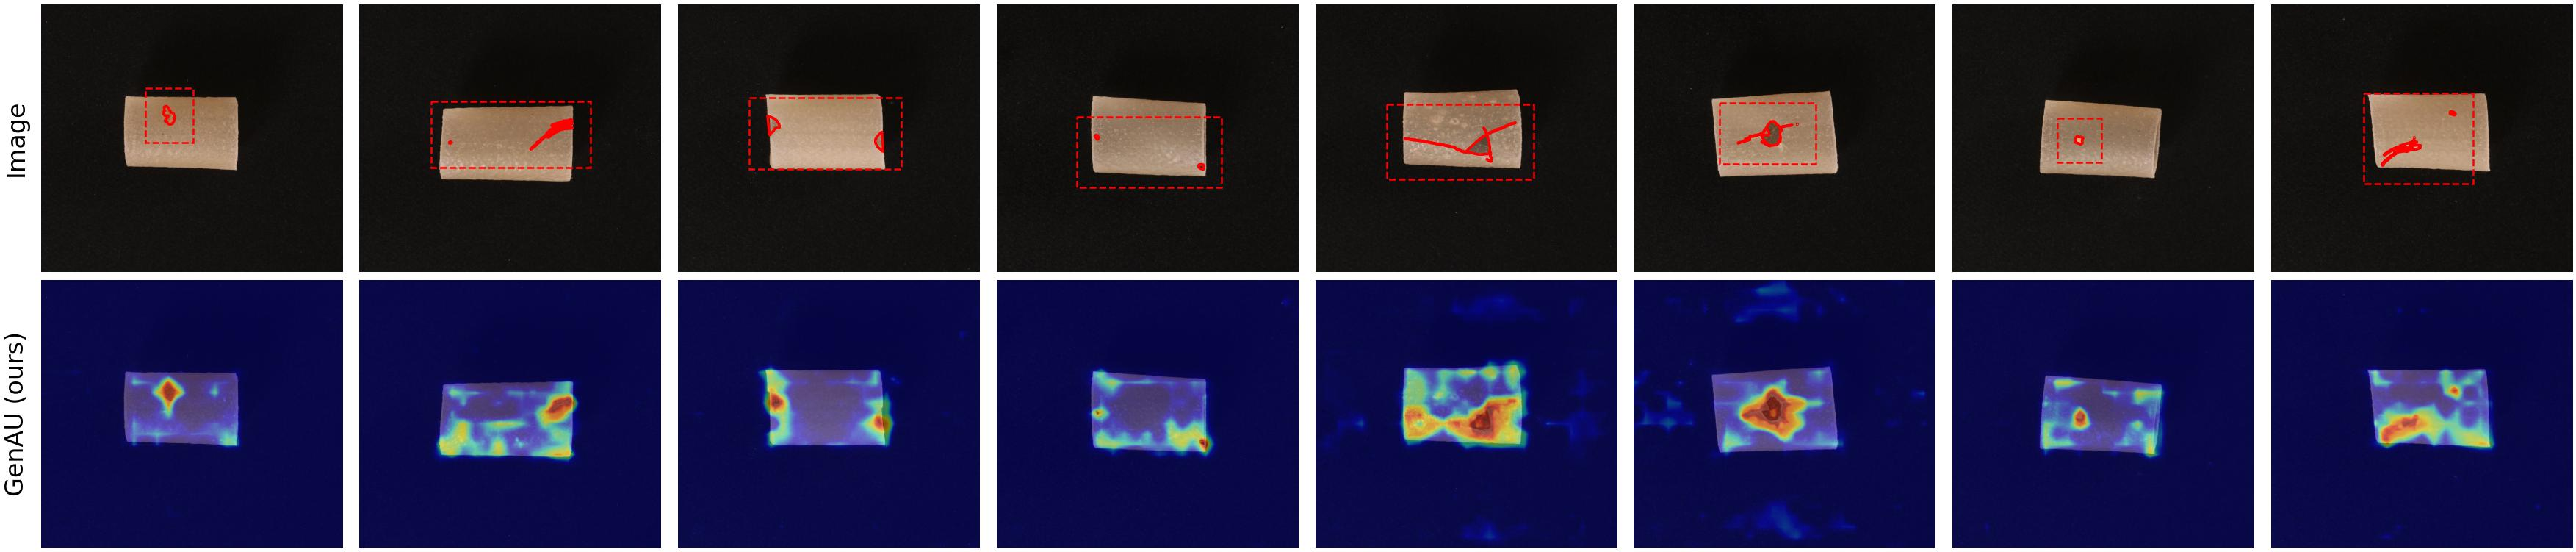
\includegraphics[width=\textwidth]{imgs/pipe-fryum.jpg}
  \caption{Pipe fryum (VisA). Ground truth is outlined in red (small defects are additionally marked with a dashed box); the second row shows the GenAU-7B anomaly maps.}
  \label{fig:pipe-fryum}
\end{figure*}

\begin{figure*}
  \centering
  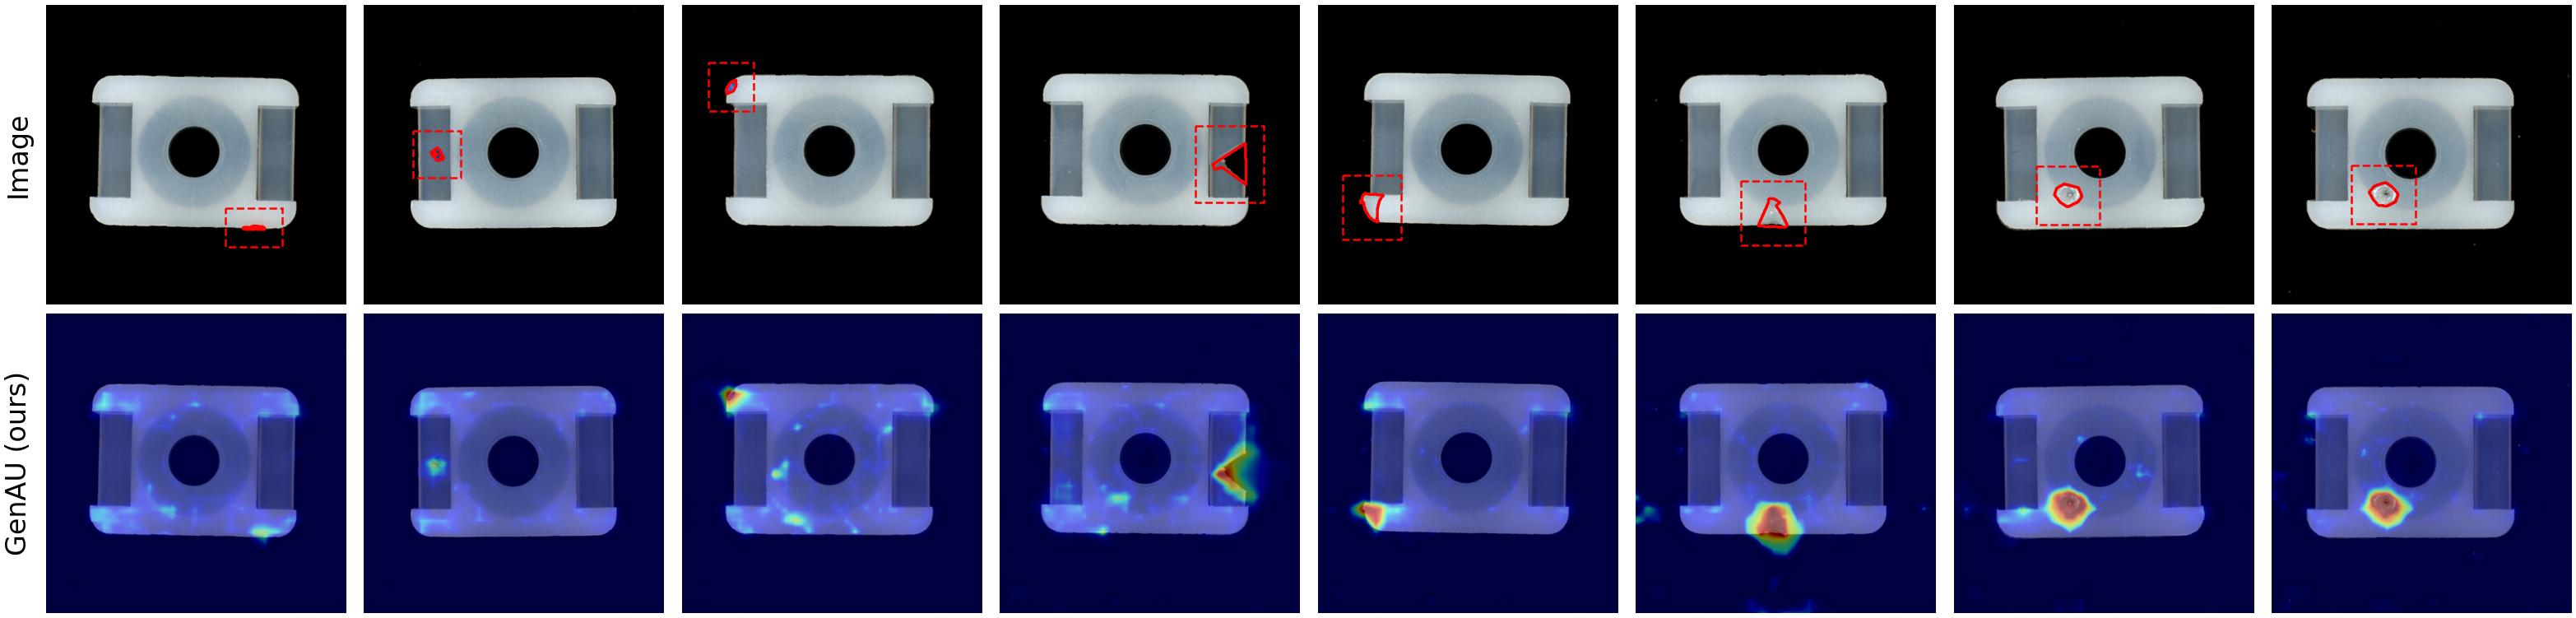
\includegraphics[width=\textwidth]{imgs/mounts.jpg}
  \caption{Mounts (Real-IAD). Ground truth is outlined in red (small defects are additionally marked with a dashed box); the second row shows the GenAU-7B anomaly maps.}
  \label{fig:mounts}
\end{figure*}

\begin{figure*}
  \centering
  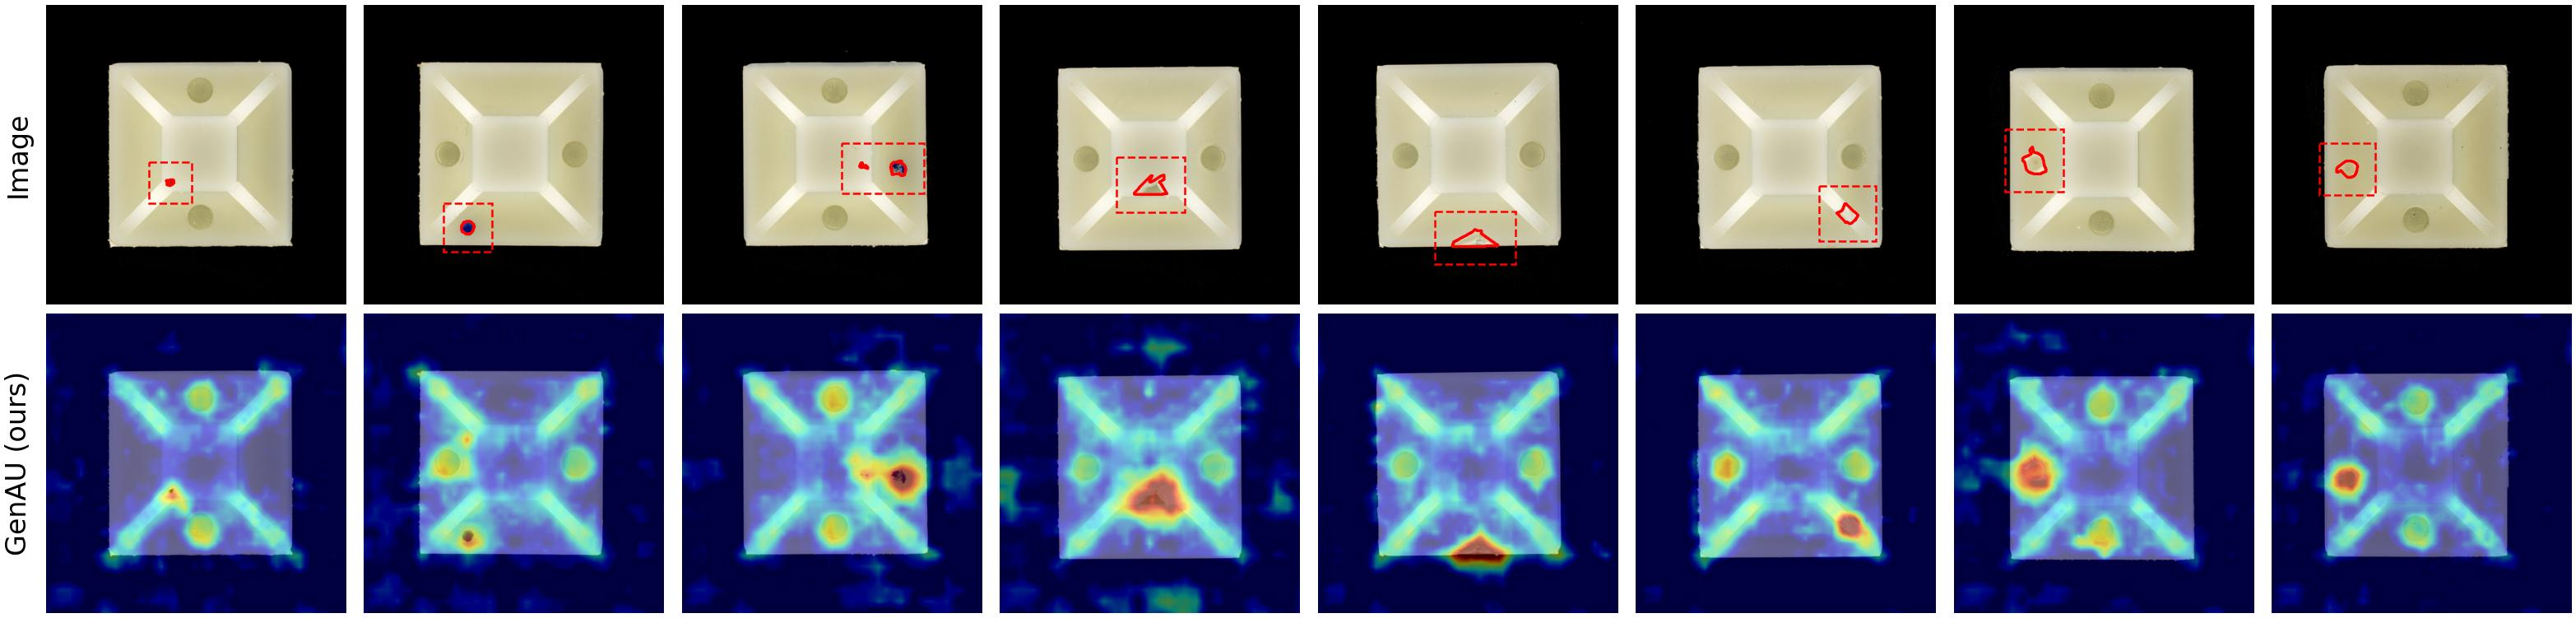
\includegraphics[width=\textwidth]{imgs/rolled_strip_base.jpg}
  \caption{Rolled strip base (Real-IAD). Ground truth is outlined in red (small defects are additionally marked with a dashed box); the second row shows the GenAU-7B anomaly maps.}
  \label{fig:rolled_strip_base}
\end{figure*}

\newcommand{\seg}[1]{{\setlength{\fboxsep}{0.8pt}\fcolorbox{orange!70!black}{orange!12}{\scriptsize\ttfamily #1}}}
\newcommand{\dlguser}[1]{\par\noindent{\setlength{\fboxsep}{2.5pt}\fcolorbox{black!35}{black!4}{\parbox{\dimexpr\linewidth-2\fboxsep-0.8pt}{\scriptsize\textbf{User:} #1}}}\par\vspace{1.5pt}}
\newcommand{\dlggenau}[2]{\par\noindent{\setlength{\fboxsep}{2.5pt}\fcolorbox{green!45!black}{green!6}{\parbox{\dimexpr\linewidth-2\fboxsep-0.8pt}{\scriptsize\textbf{GenAU:} #1\hfill{\color{black!55}[GPT-4o: #2]}}}}\par\vspace{3pt}}

\begin{figure*}
  \centering
\begin{minipage}[t]{0.325\textwidth}
  {\small\textbf{Cashew (VisA)}}\\[2pt]
  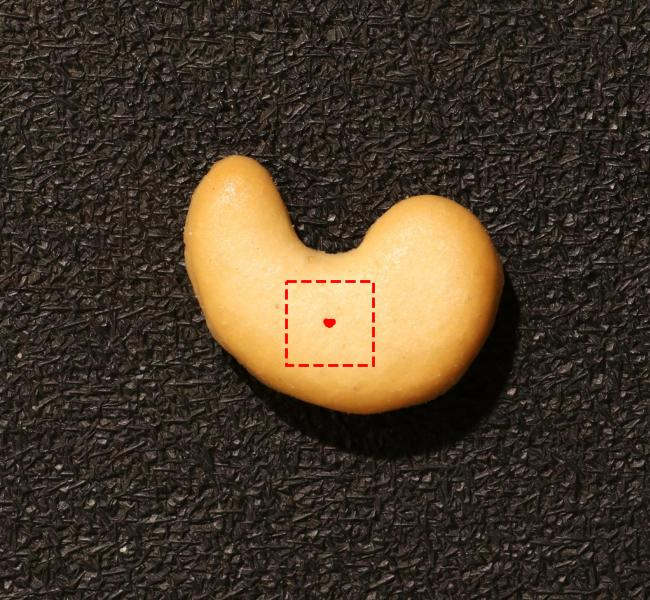
\includegraphics[width=0.495\linewidth]{imgs/a6_cashew_input.jpg}\hfill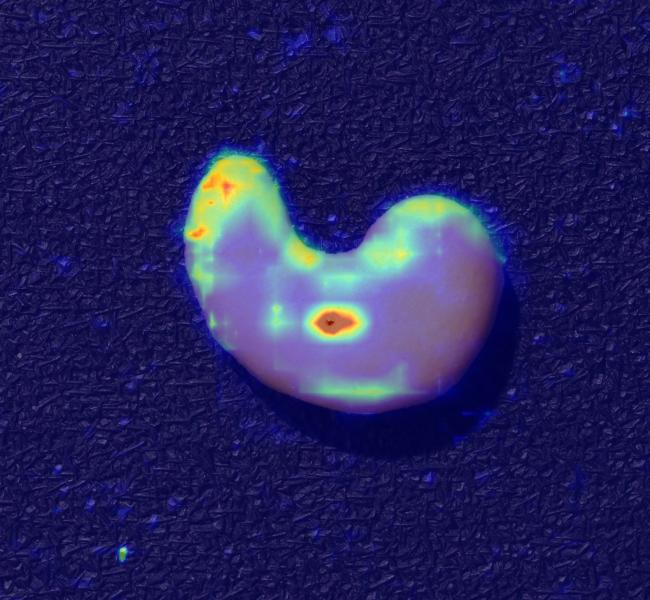
\includegraphics[width=0.495\linewidth]{imgs/a6_cashew_map.jpg}\\[3pt]
  \dlguser{Does the cashew nut in the image have any anomalies? If yes, segment it.}
  \dlggenau{Yes, there is a small, dark spot on the upper right side of the cashew nut's surface, which appears as a puncture or blemish \seg{[SEG\_defect]}~\seg{[SEG\_normal]}.}{8}
  \dlguser{Why is the hole in the cashew nut considered an anomaly?}
  \dlggenau{The hole is considered an anomaly because it disruptss the smooth, intact surface of the nut, which is typical for a healthy cashew.}{9}
  \dlguser{What might have caused the anomaly in the cashew nut?}
  \dlggenau{The anomaly could be caused by a puncture or a natural defect in the nut's shell.}{6}
  \dlguser{Can you suggest ways to prevent this kind of anomaly in cashew nuts in the future?}
  \dlggenau{To prevent such anomalies, ensure proper handling and storage to avoid physical damage. Additionally, using protective packaging during transportation can help maintain the nuts' integrity.}{5}
\end{minipage}\hfill
\begin{minipage}[t]{0.325\textwidth}
  {\small\textbf{Pipe fryum (VisA)}}\\[2pt]
  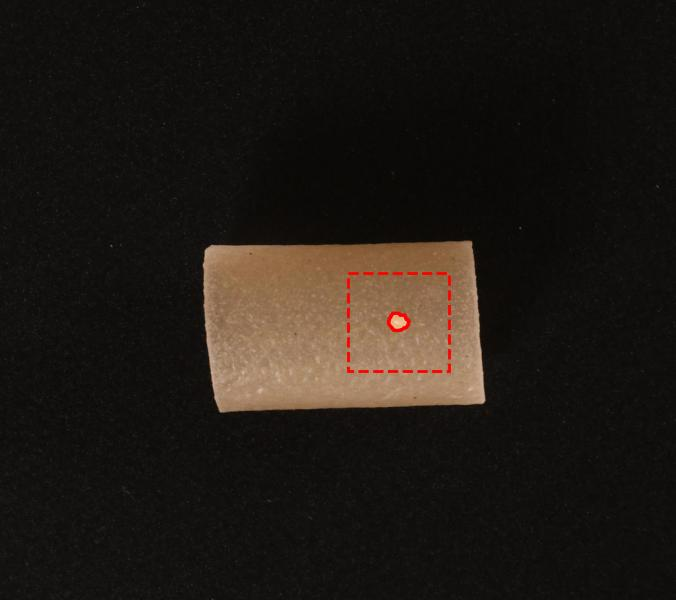
\includegraphics[width=0.495\linewidth]{imgs/a6_fryum_input.jpg}\hfill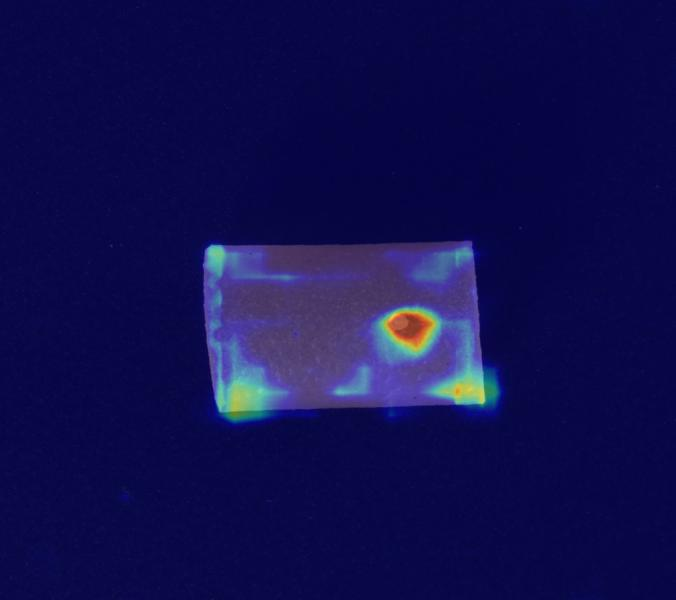
\includegraphics[width=0.495\linewidth]{imgs/a6_fryum_map.jpg}\\[3pt]
  \dlguser{Is there any anomaly visible in the image? If yes, segment it.}
  \dlggenau{Yes, there is an anomaly. A small, light-colored spot is visible on the upper right section of the pill \seg{[SEG\_defect]}~\seg{[SEG\_normal]}.}{8}
  \dlguser{What makes this spot on the fryum an anomaly?}
  \dlggenau{The anomaly is a small, light-colored spot that contrasts with the pill's uniform color.}{1}
  \dlguser{What could have caused this spot to appear on the fryum?}
  \dlggenau{The spot could be due to contamination, a manufacturing defect, or an external substance adhering to the pill.}{8}
  \dlguser{What steps can be taken to prevent such anomalies in the future?}
  \dlggenau{Enhancing quality control during manufacturing, ensuring cleanliness and sterility, and conducting regular inspections can help prevent such anomalies.}{9}
\end{minipage}\hfill
\begin{minipage}[t]{0.325\textwidth}
  {\small\textbf{PCB (VisA, pcb3)}}\\[2pt]
  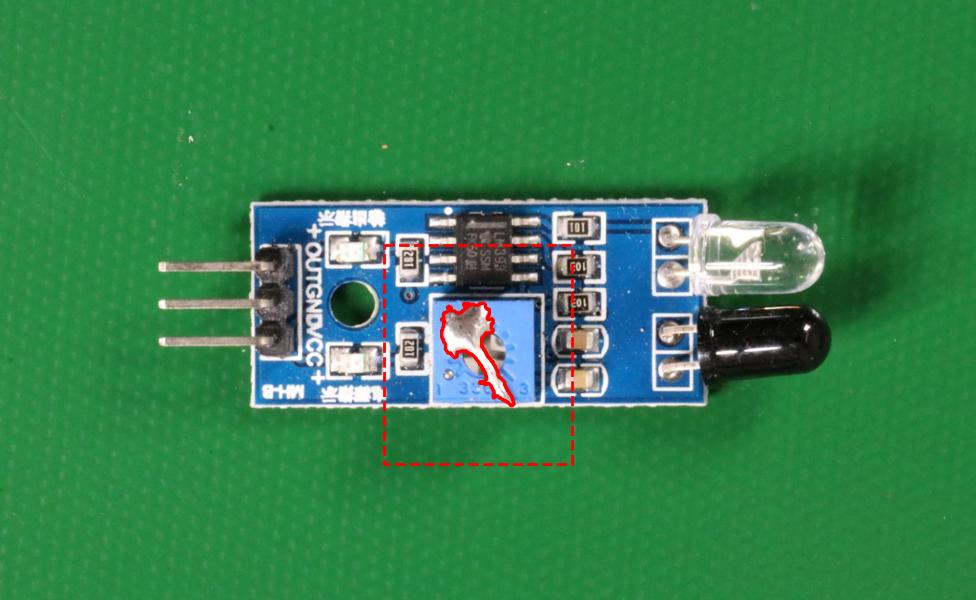
\includegraphics[width=0.495\linewidth]{imgs/a6_pcb_input.jpg}\hfill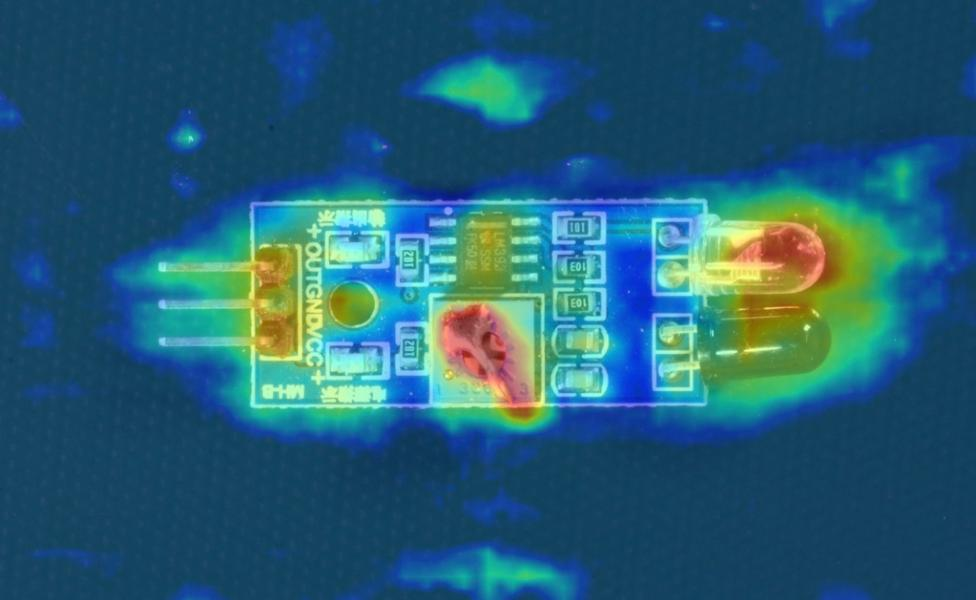
\includegraphics[width=0.495\linewidth]{imgs/a6_pcb_map.jpg}\\[3pt]
  \dlguser{Are there any observable anomalies in the PCB image? If yes, segment it.}
  \dlggenau{Yes, there is an anomaly involving the transistor on the board. The transistor's lead is bent and appears damaged, which could disrupt its functionality \seg{[SEG\_defect]}~\seg{[SEG\_normal]}.}{1}
  \dlguser{Why is the excessive solder considered an anomaly?}
  \dlggenau{The excessive solder is considered an anomaly because it can lead to short circuits, improper connections, or overheating issues.}{8}
  \dlguser{What could be the cause of this soldering error?}
  \dlggenau{The excessive solder could be caused by improper handling of the soldering iron, insufficient cooling, or a lack of experience in soldering.}{8}
  \dlguser{What measures could be implemented to prevent such anomalies?}
  \dlggenau{To prevent such anomalies, it's important to use proper soldering techniques, ensure the board is well-ventilated, and use a soldering iron with a temperature control feature.}{6}
\end{minipage}
  \caption{VisA-D\&R conversations of GenAU-7B, verbatim (including errors) from the run scored in Table~4 of the main paper. For each class we show the conversation at the class-median GPT-Score among those whose first answer reports an anomaly; [GPT-4o: $s$] is the judge's score of each answer against the reference ($1$--$10$). Left image: input with the ground truth outlined in red (dashed box around small defects); right image: the anomaly map read out from the segmentation tokens of the first answer, in a re-run of that turn on the same input. Segmentation tokens emitted in later answers are omitted.}
  \label{fig:text}
\end{figure*}



{
    \small
    \bibliographystyle{ieeenat_fullname}
    \bibliography{custom}
}

\end{document}
